\documentclass{article}
\usepackage[utf8]{inputenc}
\usepackage[spanish]{babel}
\usepackage{listings}
\usepackage{graphicx}
\graphicspath{ {images/} }
\usepackage{cite}

\begin{document}

\begin{titlepage}
    \begin{center}
        \vspace*{1cm}
            
        \Huge
        \textbf{Desafío}
            
        \vspace{0.5cm}
        \LARGE
        Ejercicio sobre instrucciones.
            
        \vspace{1.5cm}
            
        \textbf{Yuribia Viviana Arroyave}
            
        \vfill
            
        \vspace{0.8cm}
            
        \Large
        Departamento de Ingeniería Electrónica y Telecomunicaciones\\
        Universidad de Antioquia\\
        Medellín\\
        Marzo de 2021
            
    \end{center}
\end{titlepage}

\tableofcontents
\newpage
\section{Introduccción}\label{intro}
En el presente trabajo se documenta la solución a un desafío sobre la manera de dar instrucciones para llevar unos  objetos, dos trajetas y una hoja de papel, desde una posición inicial hasta una posición final.

\section{Contenido} \label{contenido}
El desafío consiste en llevar los objetos: dos tarjetas y una hoja de papel desde la posición A a la posición B siguiendo unas instrucciones dadas, dichas instrucciones fueron llevadas a cabo por tres personas diferentes con el fin de comprobar qué tan eficiente es la solución brindada. El ejercicio se encuentra documentado en un vídeo.
\vspace{0.8cm}

Posición A: Ambas tarjetas están de plano sobre un superfie una sobre la otra, y sobre ellas una hoja de papel.

\vspace{0.8cm}

Posición B: Ambas tarjetas se hallan sobre la hoja de papel formando un triángulo, donde la base es el ppel y las tarjetas son los lados del triángulo.

\subsection{Instrucciones}

\vspace{0.2cm}

\begin{itemize}
\item Hacer todo con una sola mano.
\item Tomar la hoja y correrla, dejando por fuera las tarjetas.
\item Poner ambas tarjetas sobre la hoja, una tarjeta sobreponiendo a la otra.
\item Con los dedos indice y pulgar tomar ambas tarjetas por uno de los lados más cortos.
\item Levantar las tarjetas en forma vertical, la mano queda hacia arriba y las tarjetas por el lado opuesto a la mano, quedan sobre la hoja de papel.
\item Sin soltar el indice y pulgar, poner uno de los otros dedos en medio de ambas tarjetas por uno de los lados.
\item Ir separandolas suavemente en el extremo la inferior hasta formar un triángulo, ayudarse con los otros dedos.
\item Soltar las tarjetas cuando éstas formen un triángulo que se pueda sostener.
\end{itemize}
\subsection{Evidencia en vídeo}
El vídeo con la evidencia del presente ejercicio está alojado en la página web www.youtube.com, y su enlace directo es:
https://youtu.be/ClHFobs1Swc

\newpage


\section{Imágenes} \label{imagenes}


\begin{figure}[h]
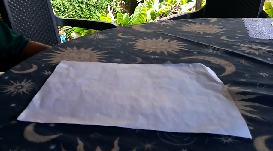
\includegraphics[width=6cm]{pos_a.png}
\centering
\caption{Posición A}
\label{fig:pos_a}
\end{figure}


\begin{figure}[h]
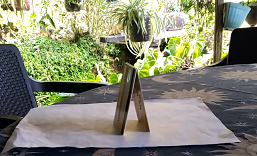
\includegraphics[width=6cm]{pos_b.png}
\centering
\caption{Posición B}
\label{fig:pos_b}
\end{figure}

\section{Conclusiones} \label{conclusiones}

Al momento de solucionar un problema es importante tener claridad sobre el problema que se quiere resolver,  y trazarse un objetivo al que se debe llegar con la solución propuesta.
\vspace{0.8cm}

Los pasos o instrucciones que deben llevar a cabo para dar solución a un problema deben darse en un lenguaje claro y preciso, para que su interpretación pueda ser la correcta y así llevar a cabo una solución eficiente.
\vspace{0.8cm}

Las pruebas son muy importantes en el desarrollo de soluciones eficientes, ya que permiten encontrar fallas en las instrucciones y así modificarlas oportunamente.



\end{document}
